\chapter{Diffusion Modeling}
\label{App:Diffusion}

\section{PDGF Modeling}
The PDGF signaling parameters are taken from an analysis performed by Lauffenburger \etal\ \cite{Lauffenburger:1989fy}. The threshold sensing concentration is based on the dissociation constant of PDGF given as, K$_{d}$ = 10$^{-10}$ - 10$^{-9}$ [mol/L]. The production rate, q$_{PDGF}$, is given as 10$^{-16}$ - 10$^{-15}$ [g/cell/min] which was cited as being taken from Leof \etal\ \cite{LEOF:1986uq}, a study using human foreskin fibroblasts. The molecular weight was estimated to be 30 [kDa]. Using the molecular weight we can convert the units of q$_{PDGF}$ to yield 5e-16/(30000*60) = 2.78e-22 [mol/cell/s]. The Einstein-Stokes equation gives $D$ = 79 [\textmu m$^{2}$/s] for the 30 [kDa] molecule.

\section{EGF Modeling}
EGF modeling was taken from work by Knauer \etal \cite{KNAUER:1984fj} and Starbuck \etal \cite{STARBUCK:1992kl}. This work is based on data obtained using human and mouse fibroblasts. The EGF complex internalization rate constant, k$_{eC}$, was measured to be  5.3e-3 [s$^{-1}$]. Half maximal response occurs at 0.15 [ng/mL] and 2000 surface complexes per cell. This means an internalization rate of 2000*5.3e-3 = 10.6 [molecules/cell/s]. The molecular weight of EGF and the EGF\slash EGF binding protein complex were cited as 6.4 and 74 [kDa] respectively. Converting units we get a 10.6/6.022e23 = 1.76e-23 [mol/cell/s] EGF uptake rate for fibroblast cells. Thus, $q_{max}$ = 2*1.76e-23 = 3.52e-23 [mol/cell/s]. Cellular affinity for EGF is about 4.69e-11 [mol/L] vs. a K$_{d}$ of 4.7e-9 [mol/L]. Again, using the Einstein-Stokes equation, a 6.4 [kDa] molecule gives a diffusion coefficient of D = 131 [\textmu m$^{2}$/s] and 58 [\textmu m$^{2}$/s] for a 74 [kDa] molecule. The latter is used to estimate the diffusing protein.

Factor uptake, q, is assumed to follow the Michaelis-Menten kinetics with respect to the concentration of a rate limiting factor (Eq \ref{App:Diffusion:equ:uptakeRate}). The value $q_{max}$ represents the maximum uptake rate per cell. $C_{cb}$ is the concentration of factor at the cell boundary and $C_{th}$ is the Monod or Michaelis-Menten constant. Per the definition of the Michaelis-Menten constant (Eq \ref{App:Diffusion:equ:uptakeRate}), when $C_{cb} = C_{th}$ then $q = q_{max}/2$. Thus, we use the threshold sensing concentration for the Michaelis-Menten constant. Therefore, when concentration at the cell boundary is 0, there is no uptake of factor, while at $C_{th}$, uptake is $q_{max}/2$.

\begin{equation}
\label{App:Diffusion:equ:uptakeRate}
q = \frac{q_{max}C_{cb}} {C_{th}+C_{cb}} = \frac{q_{max}} {1+\frac{C_{th}}{C_{cb}}}
\end{equation}

%\section{Basic geometries}
%\begin{figure}[!t]
%\centering
%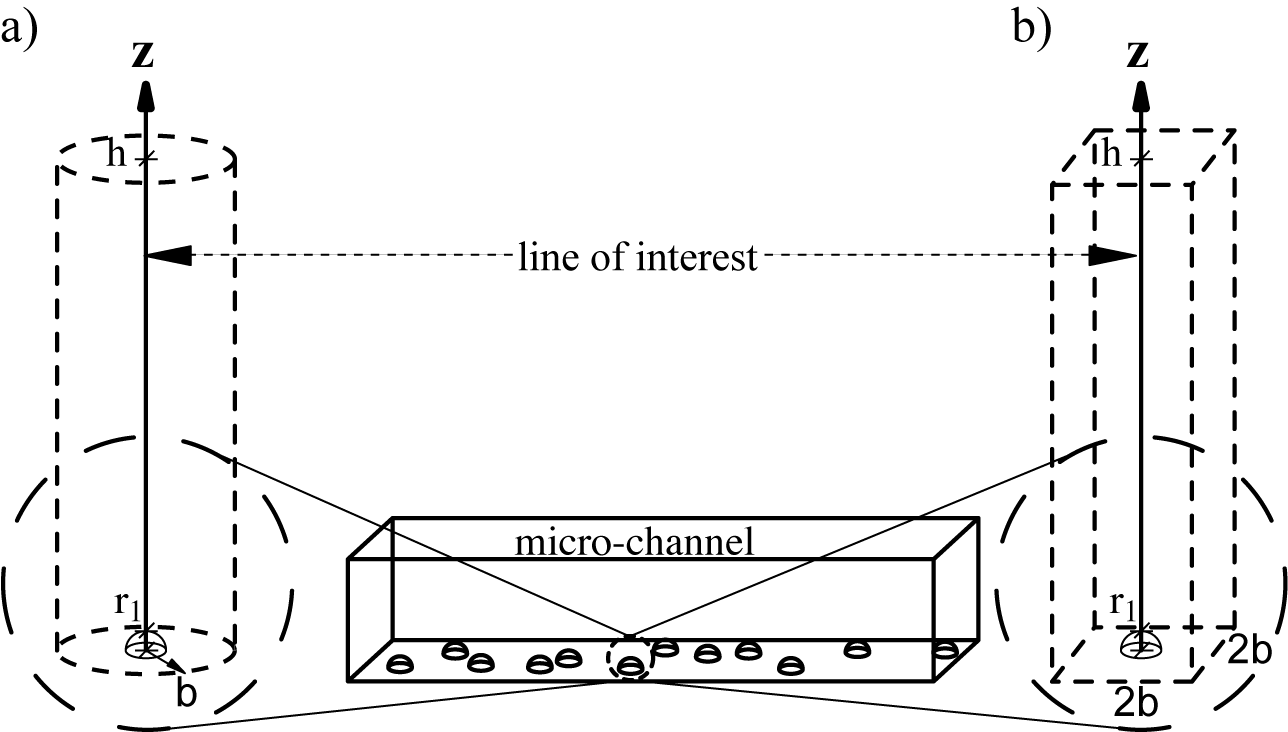
\includegraphics[width=3.5in]{Average_Geometries.pdf}
%\caption{Schematic representation of the cylindrical and rectangular geometry used to estimate the case of a single cell in culture with neighbors on a 2-D substrate. The area of the base of the unit-cylinder and unit-rectangle is equal to the area-per-cell on the substrate of the channel.}
%\label{App:Diffusion:diffusionGeom}
%\end{figure} 
%
%The line of interest labeled in Fig \ref{App:Diffusion:diffusionGeom} is the line on which a solution for the concentration will be approximated. The various ratios of the base dimension ($b$) to the height ($h$) and cell radius ($r_{1}$) will be accounted for in the boundary conditions of the one-dimensional approximation. The base dimension of the average volume is calculated from the average area per cell and the geometry. The cell is pictured as a hemisphere of radius $r_{1}$.  Items of interest emitted from or absorbed by the cell could include viruses, growth factors, cytokines, waste, or gas and have a wide range of diffusivities. The local environment of the cell has zero flux on all the walls where, on average, adjacent cells are assumed to be producing the same molecule at approximately the same rate.  An arbitrary boundary condition can be imposed at the top of the channel, $z=h$. However, we are restricted to a zero flux boundary condition at the bottom surrounding the cell, $z=0$.
%
%\section{Approximation Method}
%FE models of the average volume show that there appear to be two important regions of the model. The spherically shaped region closest to the cell and the very linear region extending far from the cell along the line of interest. These observations suggest it might be possible to add the solution of a spherical system that only depends on the radius, $r$, with a one-dimensional solution in Cartesian coordinates to obtain a total solution with sufficient accuracy to model the average cellular microenvironment (see Fig \ref{App:Diffusion:boundaries}). The idea of a linear combination to obtain the approximation is shown in Eq \ref{equ:linAdd} where $\alpha$ and $\beta$ represent the weighting of the terms in the total solution. As an addition note, other methods other than a simple linear addition were investigated, such as those that would transition between the solutions or vary the weighting with distance along the line of interest, yet they produced only slightly better results with the disadvantage of added complexity. Subscript $a$ refers to the approximation obtained from the one-dimensional solutions. Subscript $s$ refers to the one-dimensional spherical system and $c$ refers to the one-dimensional Cartesian system.
%
%\begin{figure}[!ht]
%\centering
%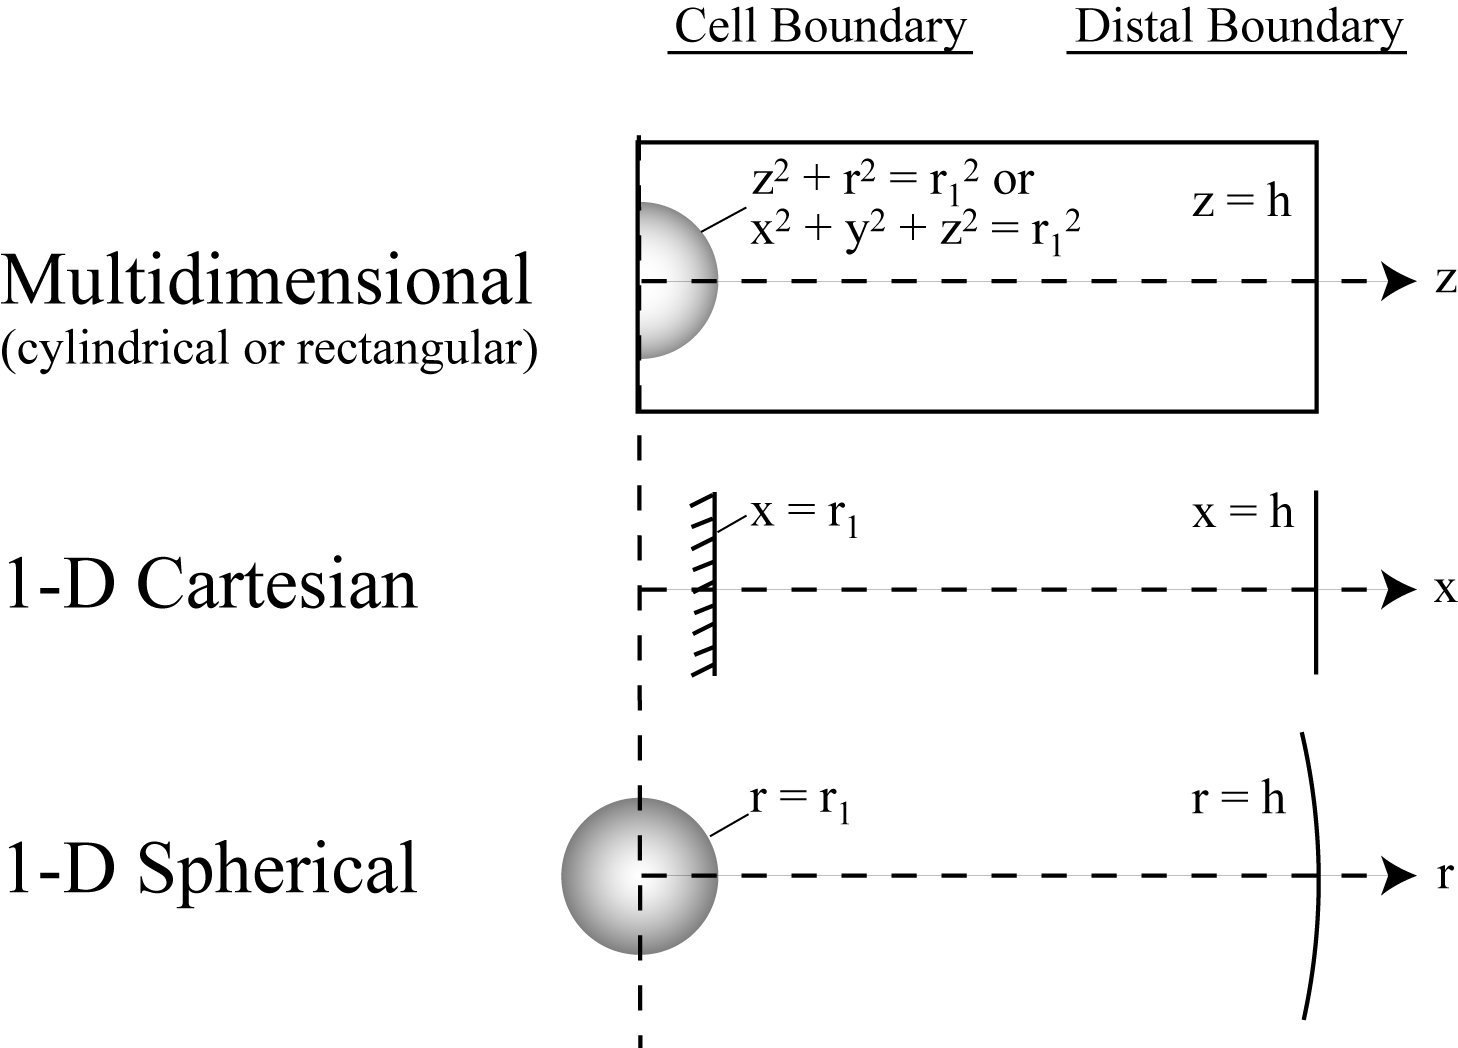
\includegraphics[width=3.5in]{Diffusion_Boundaries.pdf}
%\caption{Coordinate systems for the multidimensional models as well as the one-dimensional models.}
%\label{App:Diffusion:boundaries}
%\end{figure}
%
%
%\begin{equation}
%C_{a} = \alpha \, C_{s} + \beta \, C_{c}
%\label{equ:linAdd}
%\end{equation}
%
%Two conditions were imposed on the boundary conditions of the one-dimensional solutions to effectively determine $\alpha$ and $\beta$. The first condition was the conservation of mass. The change in average concentration with time for the volume must be the same between the multidimensional model and the approximation, as shown in Eq \ref{equ:balMass}. The second imposed condition is that the sum of the concentration gradients used in the one-dimensional system must equal the concentrations gradient perpendicular to cell boundary in the multidimensional model. The second condition is shown in Eq \ref{equ:balGrad} where $\overrightarrow{n}$ is the unit vector that points outward normal to the cell surface. Subscript $m$ refers to the multidimensional system in which all geometry is modeled precisely. 
%
%\begin{equation}
%\frac{d \overline{C}_{m}}{ d t} = \frac{ d \overline{C}_{s}}{ d t} + \frac{ d \overline{C}_{c}}{ d t}
%\label{equ:balMass}
%\end{equation}
%
%\begin{equation}
%\left( \frac{\partial C_{m}}{ \partial n} =  \frac{ \partial C_{s}}{ \partial r} + \frac{ \partial C_{c}}{ \partial x} \right) \Big |_{\textrm{\tiny cell boundary}}
%\label{equ:balGrad}
%\end{equation}
%
%By combining these conditions, the following equations for the flux boundary condition at a given time is as follows.
%
%\begin{equation}
%\label{equ:gradCart}
%\left(\frac{\partial{C_{c}}}{\partial{x}} = \frac{\partial C_{m}}{ \partial n}  \frac{ \mu-\eta}{\mu-\frac{1}{h-r_{1}}}\right) \Big |_{\textrm{\tiny cell boundary}}
%\end{equation}
%
%\begin{equation}
%\label{equ:mu}
%\mu=\frac{-3r_{1}^{2}}{h^{3}-r_{1}^{3}}
%\textrm{, and}
%\end{equation}
%
%\begin{equation}
%\label{equ:eta}
%\eta=\frac{-2\pi r_{1}^{2}}{\pi b^{2}h-\frac{2}{3}\pi r_{1}^{3}} \textrm{   (cylindrical)}
%\end{equation}
%
%\begin{equation}
%\label{equ:eta}
%\eta=\frac{-2\pi r_{1}^{2}}{4b^{2}h-\frac{2}{3}\pi r_{1}^{3}} \textrm{   (rectangular)}
%\end{equation}
%
%Eq \ref{equ:balGrad} is then used to calculate the flux boundary condition $\partial C_{s}/ \partial r$ at the cell boundary from the solution to Eq \ref{equ:gradCart}. Eq \ref{equ:gradCart} is used to create Fig \ref{App:Diffusion:ratio} where the ratio of the boundary conditions is between 0 and 1. If the ratio is $<0$ or $>1$, then the approximation method breaks down producing opposing boundary conditions. For the cylindrical geometry the ratio is 0 when $h/b= 3/ \sqrt{6}$ and where $h/b=\sqrt{6/ \pi}$ in the case of the rectangular geometry. Similarly, the ratio is 1 when $b=r_{1}\sqrt {-6h( 2r_{1}-3h}/(3h)$ and $b=r_{1}\sqrt {-6h\pi( 2r_{1}-3h)}/(6h)$ for the cylindrical and rectangular case respectively. The ratio is used to solve the one-dimensional problems over the distance $r=r_{1}\,...\,h$ with a diffusion coefficient, $D$, for the molecule of interest.
%
%\begin{figure}[!ht]
%\centering
%\includegraphics[width=2.5in]{Ratio_080207.pdf}
%\caption{Plot of $(\partial C_{c}/ \partial x)/(\partial C_{m}/ \partial n)$ for various ratios of $b/r_{1}$ and $h/r_{1}$ for the cylindrical geometry shown in Fig Xa.}
%\label{App:Diffusion:ratio}
%\end{figure}
%
%
%\section{Results and Discussion}
%\subsection{Constant flux boundary condition}
%The FE modeling software, COMSOL (PLACE), is used in conjunction with Matlab to produce all the transient diffusion results. The accuracy of the approximation is examined first using the simple case of a constant flux boundary condition on the cell. A simulation is performed for a cell with an average cell with a diameter of 10 $\mu$m producing glucose with a diffusion coefficient $D$ = 0.0016 mm$^{2}$/s at a rate of $R$ = 5.56$\times$10$^{-6}$ nmol/cell/s in a microchannel of height $h$ = 250 $\mu$m with 300 cells/mm$^{2}$. 
%%
%%\begin{figure}[!ht]
%%\centering
%%
\includegraphics[width=2.5in]{box.jpg}
%%\caption{Plot of concentration vs. time for the cell boundary and ceiling of the microchannel for the multidimensional model, $C_{m}$, and the approximation, $C_{a}$, for the geometry shown in Fig Xb and parameters listed above.}
%%\label{App:Diffusion:graphCt}
%%\end{figure}
%
%Fig \ref{App:Diffusion:graphCt} shows how the approximation tracks with the 3-D COMSOL model. Notice that the difference between the approximation and multidimensional model grows until it stabilizes to a constant difference when the system stabilizes and uniformly raises in concentration over time according to Eq \ref{equ:balMass}. In order to present a comparison of the multidimensional model and approximation over a large range of geometric aspect ratios, the system is made dimensionless. Time is made dimensionless using Eq \ref{equ:tau}. Error will be reported as the percent difference between the multidimensional model and the approximation calculated at the cell boundary for $\tau$ = 1. The value of 1 is chosen for $\tau$ as it is indicative of the time it takes for a system to approach steady-state with constant flux boundary conditions. Error is plotted for various aspect ratios of the cylindrical geometry on a contour plot in Fig \ref{App:Diffusion:errorCyl}. The same is done for the rectangular geometry in Fig \ref{App:Diffusion:errorRect}.
%
%\begin{equation}
%\label{equ:tau}
%\tau = \frac{ \left( h - r_{1} \right) ^{2}}{2D}
%\end{equation}
%
%\begin{figure}[!ht]
%\centering
%\includegraphics[width=2.5in]{Cylindrical_080207.pdf}
%\caption{Error results for a constant flux boundary condition. Above is a plot of $100 \% \times (C_{m}-C_{a})/C_{m}$ for various ratios of $b/r_{1}$ and $h/r_{1}$ for the cylindrical geometry shown in Fig Xa.}
%\label{App:Diffusion:errorCyl}
%\end{figure}
%
%\begin{figure}[!ht]
%\centering
%
\includegraphics[width=2.5in]{/Users/warrick/Documents/Videos_and_Images/box.jpg}
%\caption{Error results for a constant flux boundary condition. Above is a plot of $100 \% \times (C_{m}-C_{a})/C_{m}$ for various ratios of $b/r_{1}$ and $h/r_{1}$ for the rectangular geometry shown in Fig Xb.}
%\label{App:Diffusion:errorRect}
%\end{figure}
%
%Results from this section suggest that the method of approximation is valid and quite accurate for a large range of aspect ratios and cell densities. Figs \ref{App:Diffusion:errorCyl} and \ref{App:Diffusion:errorRect} indicate errors typically less than 10\% in magnitude within the applicable range of aspect ratios shown in Fig \ref{App:Diffusion:ratio}. Typical microchannel heights for cell culture are many multiples of the cell radius. If a cell is roughly 10 $\mu$m in diameter, and $h/r=30$, the microchannel height is approximately 150 $\mu$m and the approximation would be appropriate where cell density is $>57$ cells/mm$^{2}$. If $h/r=50$, then the channel height would be 250 $\mu$m and the approximation would be appropriate for cell densities $>20$ cells/mm$^{2}$. Thus, the approximation is valid for many typical cell culture parameters and can be applied as the cells proliferate and approach confluency.
%
%
%\subsection{Transient flux boundary condition}
%With positive results in the case of constant flux it is now necessary to address the situation of transient flux. The flux boundary condition is made to follow a Gaussian profile over time. A Gaussian profile is determined by the value for the mean ($\bar x$), standard deviation ($\sigma$), and maximum ($y_{max}$). The profile mean is at $\tau=1.\bar3$. $\sigma$ corresponds to $0.\bar3$ units of dimensionless time, $\tau$. Thus, at $\tau=0$ the flux is at $-4\sigma$ along the Gaussian profile. This situation might approximate the transient response of a cell to a stimulus. Typical results for the two methods using a cylindrical geometry are plotted in Fig \ref{App:Diffusion:errorTime} along with a normalized plot of the flux profile. The difference between the two methods increases during the rise in concentration and then approaches zero as the system stabalizes. The percent difference in cell boundary concentration at the peak of the flux (i.e. at $\tau=1.\bar3$) between the multidimensional model and the approximation using the cylindrical geometry is reported in Fig \ref{App:Diffusion:errorTime} for various aspect ratio as a contour plot. Results show good agreement with the multidimensional model again with similar errors as the case of a constant flux boundary condition.
%
%\begin{figure}[!ht]
%\centering
%\includegraphics[width=2.5in]{Cylindrical_Transient_080207.pdf}
%\caption{Error results for a transient flux boundary condition following a Gaussian profile. Above is a plot of $100 \% \times (C_{m}-C_{a})/C_{m}$ for various ratios of $b/r_{1}$ and $h/r_{1}$ for the cylindrical geometry shown in Fig Xa.}
%\label{App:Diffusion:errorTime}
%\end{figure}
%
%
%
%
%
%
%
%
%\subsection{Dynamics of diffusion and biology}
%One typical change during \textit{in-vitro} cell culture is the cell number. A major advantage of reducing the multidimensional diffusion problem to a one-dimensional problem is that changes in cell number (i.e. the spacing parameter $b$) can be accounted for using Eq \ref{equ:gradCart}. Thus, the approximation method can accommodate changes in cell density due to cell proliferation, death, or apoptosis by adjusting the flux boundary condition accordingly. There is no need to interrupt the model and incrementally re-mesh the geometry making the FE model impractical for many users. 
%
%Through simulation one can also identify when diffusion dynamics result in significant concentration differences within the system and could possibly affect cell behavior. One way to estimate the concentration distribution within the channel is to look at a steady-state system with constant flux at the cell. At steady-state, the difference, $\triangle C$, between the concentration at the cell boundary and at the ceiling of the channel for the approximation are given by the following equations.
%
%\begin{equation}
%\label{equ:steady}
%\triangle C=\frac{\alpha}{r_{1}-h}+\frac{\beta}{2}(r_{1}^{2}-h^{2}) + \frac{h-r_{1}}{2} \left(\frac{\partial C_{c}}{\partial x} \big |_{x=r_{1}}\right)
%\end{equation}
%
%\begin{equation}
%\label{equ:alpha_2}
%\alpha = -\beta r_{1}^{3}+ r_{1}^{2} \left(\frac{\partial C_{s}}{\partial r} \big |_{r=r_{1}}\right)
%\end{equation}
%
%\begin{equation}
%\label{equ:beta_2}
%\beta = -\frac{r_{1}^{2}}{h^{3}-r_{1}^{3}} \left(\frac{\partial C_{s}}{\partial r} \big |_{r=r_{1}}\right)
%\end{equation}
%
%$\triangle C$ is affected by the dimensions of the system and the rates of influx and efflux to and from the cell. Concentration differences increase with increasing dimensions and increasing rates of flux. $\triangle C$ can be compared to other important concentration parameters of the system. For example, if the initial concentration of nutrients within a microchannel, $C_{0}$ is $\gg \triangle C$ then the dynamics of diffusion will have little relative effect on concentrations. However, if $C_{0} \sim \triangle C$ or if nutrients are depleted to a point where the average concentration, $\overline{C}$, is on the order of $\triangle C$, then the dynamics of diffusion could play an important role in system behavior. Another consideration is the relative size of $\triangle C$ to threshold concentrations of the cell, $C_{t\_i}$. If $\triangle C \ll C_{t\_i}$, then diffusion dynamics will play little role in affecting concentrations near thresholds.
%
%The time scale and biological dynamics of the system can also be important when considering the role of diffusional effects. For example, if the time scale of the biological process is on the order of $\tau$, an estimate of the time it takes for diffusion to redistribute the soluble factor (see Eq \ref{equ:tau}), the dynamics of the biological process and diffusion will interact for unique system behavior. Alternatively, even if $\triangle C$ is relatively small and $\tau$ is much less that the time scale of the biological process, effects of the concentration distribution could be significant when integrated over a large time. For example, if a soluble factor played a critical role in exponential cell growth, over time, the effects of a small difference in concentration could be greatly magnified over time. Similarly, biological processes with tight thresholds or feedback loops could be very sensitive to subtle changes in microenvironmental concentrations due to diffusional dynamics.
%
%Some of the considerations that were just discussed can be seen in a simple model of cell growth in response to a rate limiting factor. Factor concentration and cell proliferation are dynamically modeled together using Matlab and a Crank-Nicolson method for modeling diffusion.
%
%Proliferation rate is assumed to follow the Michaelis-Menten kinetics with respect to the concentration of a rate limiting factor (Eq \ref{equ:prolRate}). $u_{max}$ represents the maximum proliferation rate of the cells. $C$ is the concentration of factor at the cell boundary and $K_{m}$ is the Monod or Michaelis-Menten constant, which is the concentration at which the proliferation is at $u_{max}/2$. Population kinetics are then modeled using Eq \ref{equ:pop} where N is the cell number. Many other terms could be included into Eq \ref{equ:prolRate} to more accurately model the system such as the possible negative effects of waste concentration or cell contact inhibition. As more soluble factors are added to the system, a separate, simultaneous model of diffusion is needed to keep track of each concentration. In the interest of simplicity, extra terms are neglected in this example. The result of the simulation (the dynamic model) will be compared to a model that assumes even and constant mixing of the microchannel (the evenly-mixed model). The hypothesis is that the distribution of soluble factors can play a significant role in the dynamics of the system as a whole.
%
%\begin{equation}
%\label{equ:prolRate}
%u = \frac{u_{max}C} {K_{m}+C}
%\end{equation}
%
%\begin{equation}
%\label{equ:pop}
%u = \frac{1}{N} \frac{dN}{dt}
%\end{equation}
%
%The cell number over time is plotted for the dynamic and evenly-mixed model are plotted over time to show the difference in the results. Tab X shows simulation results for a wide variety of parameters. In some cases, there is enough factor to double the population size while in other cases, the  factor is depleted and growth rate approaches $0$. If the population doubles, the time at which it doubles is reported as $t_{2N_{0}}$. If the population growth rate falls to one tenth of the maximum growth rate, the cell number and time, $t_{u_{max}/10}$, at which it occurs are recorded. The ratio  $(\partial C_{c}/ \partial x)/(\partial C_{m}/ \partial n$) is always between 0 and 1 in the simulations. Also $b/r$ is always $>1$. Corresponding values of $\triangle C$ and $\tau$ are given for later analysis and discussion. The time scale of the biological process is estimated here as the doubling time of the cell population when the proliferation rate is at a maximum and is referred to using $t_{bp}$.